\begin{align}
 \tag{5.12.1}
 \pr{X} = 
  \begin{cases}
    0, & \text{for }  X = 0 \\
    k, & \text{for }  X = 1 \\
    2k, & \text{for } X = 2 \\
    2k, & \text{for } X = 3 \\
    3k, & \text{for } X = 4 \\
    k^2, & \text{for } X = 5 \\
    2k^2, & \text{for } X = 6 \\
    7k^2 + k, & \text{for } X = 7 \\
    \end{cases}
  \end{align}
\begin{enumerate}
    \item It is known that the sum of probabilities of a probability distribution is always one. 
\begin{align}
\tag{5.12.2}
    \therefore 0 + k + 2k + 3k + k^2 + 2k^2 + (7k^2 + k) = 1 
\end{align}
\begin{align}
\tag{5.12.3}
\implies 10k^2 + 9k - 1 = 0 
 \implies  (10k - 1)(k + 1) = 0
 \end{align}
 
  \begin{equation}
  \tag{5.12.4}
 \implies  k = -1, \frac{1}{10} 
\end{equation}
\begin{equation}
    \tag{1}
 \therefore k = \frac{1}{10} (\because k \ge 0)
 \end{equation}
 
%  \begin{figure}[!htb]
%     \centering    
% 	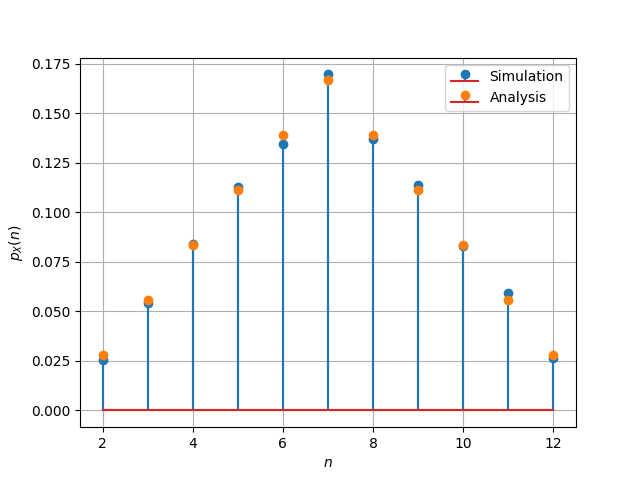
\includegraphics[width=\columnwidth]{pmf.png}
%     \caption{Probability Mass Function(PMF)}
%     \label{Fig:1}
% \end{figure}

% \begin{figure}[!htb]
%     \centering    
% 	\includegraphics[width=\columnwidth]{cdf.png}
%     \caption{Cumulative Distribution Function(CDF)}
%     \label{Fig:2}
% \end{figure}
 \begin{table}[]
\begin{tabular}{|l|l|l|l|l|l|l|l|l|}
\hline
X    & 0 & 1   & 2   & 3   & 4   & 5    & 6    & 7 \\ \hline
F(X) & 0 & 0.1 & 0.3 & 0.5 & 0.8 & 0.81 & 0.83 & 1 \\ \hline
\end{tabular}
\caption{CDF of X}
\end{table}
 We know that \pr{X \le x} = F(x) \\
 and  \pr{x< X \le y} = F(y) - F(x) \\
\item \pr{X < 3} = \pr{X \le 3} - \pr{X = 3} 
 \begin{align}
 \tag{5.12.5}
 \implies \pr{X < 3} =F(3)- \pr{X = 3} \\
\tag{5.12.6}
\implies  \pr{X < 3} = \frac{5}{10} - \frac{2}{10}   \\
\tag{2}
\therefore  \pr{X < 3} = \frac{3}{10} 
   \end{align} 
 \item \pr{X > 6} = 1 - \pr{X \le 6} = 1 - F(6)
 \begin{align}
\tag{5.12.7}
\implies  \pr{X > 6}  = 1 - \frac{83}{100} \\
\tag{3}
\therefore \pr{X > 6} = \frac{17}{100} 
\end{align}
\item \pr{0 < X < 3} = \pr{0 < X \le 3} - \pr{X = 3}  
\begin{align}
\tag{5.12.8}
\implies \pr{0 < X < 3} = F(3) - F(0) - \pr{X = 3} \\
 \tag{5.12.9}
\implies   \pr{0 < X < 3} = \frac{5}{10} - 0 - \frac{2}{10} \\
\tag{4}              
    \therefore    \pr{0 < X < 3} = \frac{3}{10}
\end{align}

\end{enumerate}